%-------------------------------------------------------------------------------
\section{Introduction}
%-------------------------------------------------------------------------------

%-------------------------------------------------------------------------------
\section{Results}
%-------------------------------------------------------------------------------

\subsection{Coherence}

Spectral coherence is the Fourier analogue of linear correlation.
We computed the coherence between the \SIrange{31.3}{97.8}{Hz} range for pairs of depths.
Coherence between channels was computed using the Welch method using \SI{256}{\milli\second} windows with \SI{50}{\percent} overlap.

\begin{figure}[htb]
    \centering
    \subfloat[][\label{fig:lam_coher_lfp}]{
        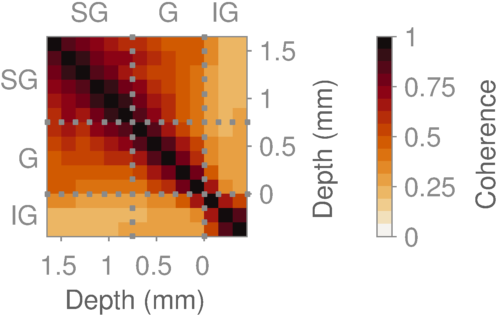
\includegraphics[width=0.47\linewidth]{coherence/coherence-avg_paper_Cln.png}
}
    ~~
    \subfloat[][\label{fig:lam_coher_csd}]{
        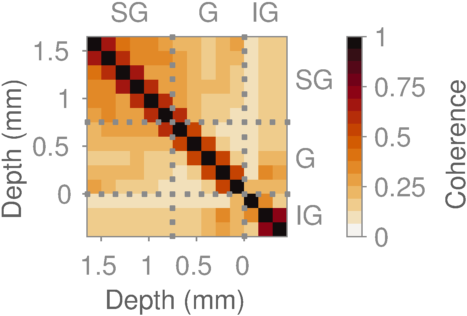
\includegraphics[width=0.47\linewidth]{coherence/coherence-avg_paper_Csd.png}
}
    \caption{Coherence \SIrange{31.3}{97.8}{Hz}
\protect\subref{fig:lam_coher_lfp}:~\ac{LFP}.
\protect\subref{fig:lam_coher_csd}:~\ac{CSD}.
}
\label{fig:lam_coher}
\end{figure}

The results show the same compartmentalisation as we observed for the information redundancy in the high frequency range, namely that \ac{G} and \ac{SG} are more correlated in the higher frequency ranges than they are with \ac{IG}.

The results for the coherence of the \ac{LFP} (Fig.~\ref{fig:lam_coher_lfp}) show more coherence than the \ac{CSD} (Fig.~\ref{fig:lam_coher_csd}).
This is to be expected since the \ac{CSD} is a better representation of the current sources within the cortex, whose broad extent induces voltage differences (and hence \ac{LFP}) across a larger amount of cortex.

Our results are in agreement with the observations of \citet[Figure 5B]{Maier2010}.


%-------------------------------------------------------------------------------
\subsection{Signal and Noise Correlation}

\marginpar{Take text from supplemental materials for paper, but here with the addition of phase correlating with itself and with power.}

\begin{figure}[htb]
    \centering
    \subfloat[][\label{fig:lam_signal_corr_depth}]{
        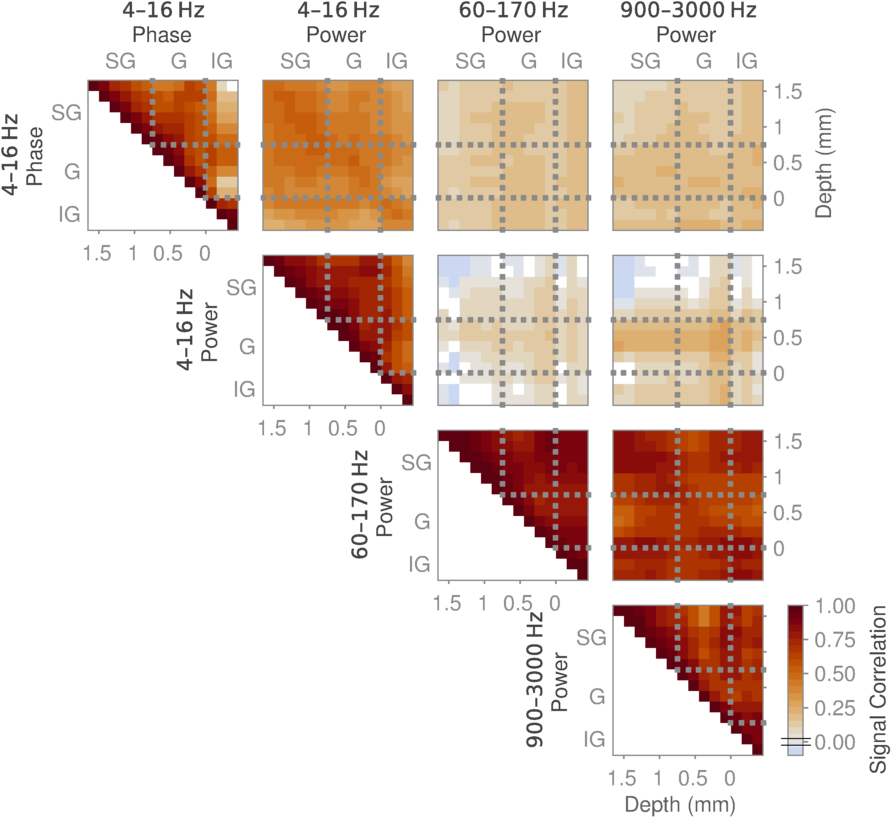
\includegraphics[width=0.47\linewidth]{noisesigcorr/bndflt4-signal-avg_paper.png}
}
    ~~
    \subfloat[][\label{fig:lam_noise_corr_depth}]{
        %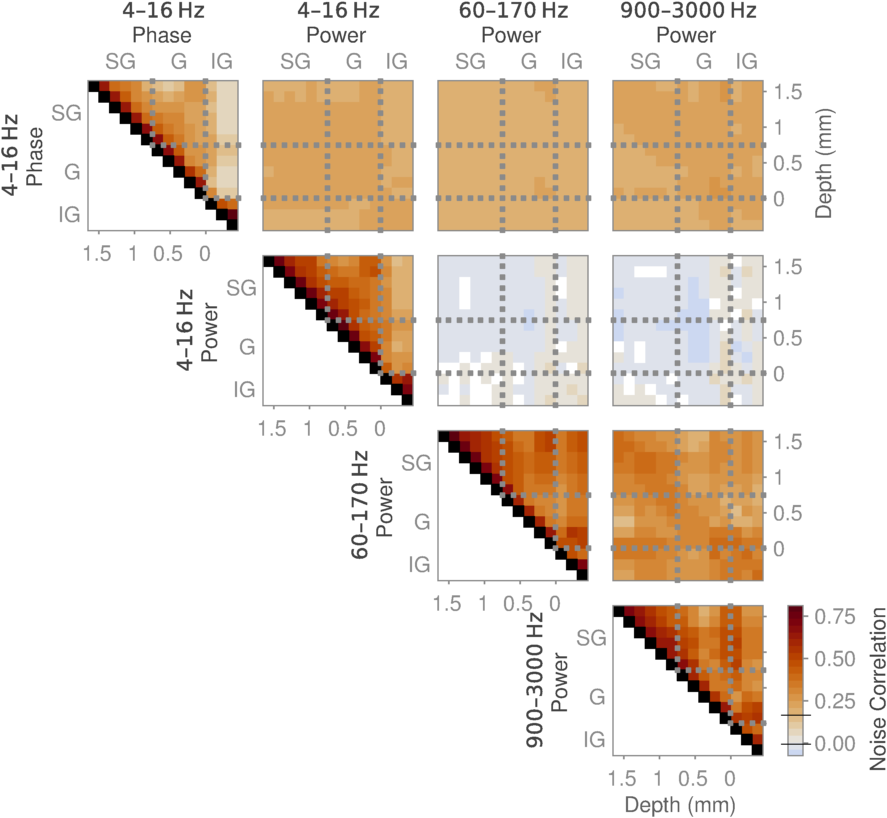
\includegraphics[width=0.47\linewidth]{noisesigcorr/bndflt4-noise-avg_paper.png}
        <Code running>
}
    \caption{
\protect\subref{fig:lam_signal_corr_depth}:~Signal correlation.
\protect\subref{fig:lam_noise_corr_depth}:~Noise correlation.
}
\label{fig:lam_noisesignal_corr_depth}
\end{figure}


\begin{figure}[htb]
    \centering
    \subfloat[][\label{fig:lam_signal_corr_phase}]{
        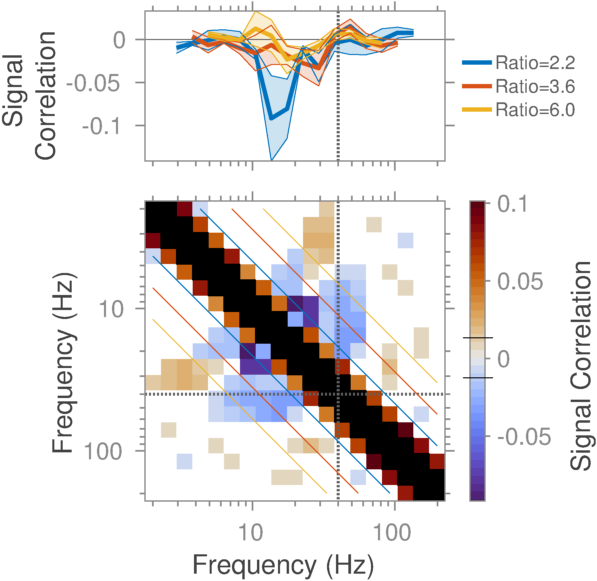
\includegraphics[width=0.47\linewidth]{noisesigcorr/cxsfrq-signal-phase-phase-avg-log.png}
}
    ~~
    \subfloat[][\label{fig:lam_noise_corr_phase}]{
        %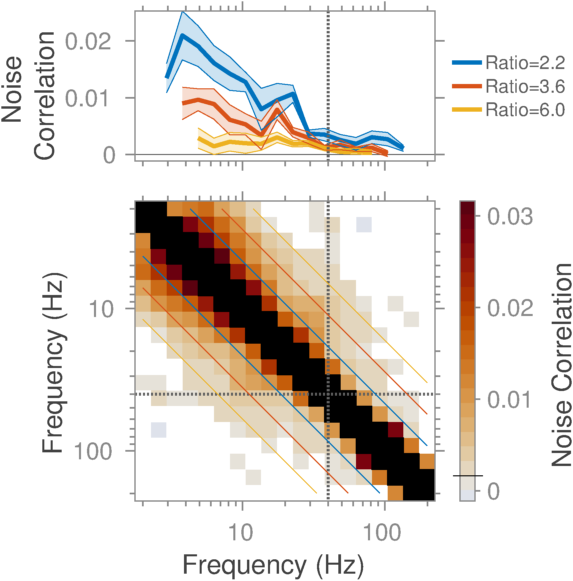
\includegraphics[width=0.47\linewidth]{noisesigcorr/cxsfrq-noise-phase-phase-avg-log.png}
        <Code running>
}
    \caption{Phase correlation
\protect\subref{fig:lam_signal_corr_phase}:~Signal correlation.
\protect\subref{fig:lam_noise_corr_phase}:~Noise correlation.
}
\label{fig:lam_noisesignal_corr_phase}
\end{figure}

Circular statistics were computed using the CircStat toolbox \citep{Berens2009}.

%-------------------------------------------------------------------------------
\section{Discussion}
%-------------------------------------------------------------------------------
